% L12a minority game, two panels (November 5, 2026; the instructor's NSF-proposal figure
% was the starting point). A: one round, with both feedback paths (the minority action
% into the history, the attendance into every strategy's score). B: one agent's two
% strategy tables for m = 3, the current history row, the scores, and the Boltzmann
% probabilities at T equal to the score gap.
%
% Consistency checks (by hand): history window (-1, +1, +1) is row 4 of the table;
% the drawn actions -1, +1, -1 sum to -1 < 0, so the minority action is +1; in row 4,
% strategy 1 plays -1 (majority) and strategy 2 plays +1 (minority), so U_i2 rises and
% U_i1 falls under U(t+1) = U(t) - a A(t)/P with A(t) < 0; scores 2.4 and 0.9 give a gap
% of 1.5, and at T = 1.5 the probabilities are e/(e+1) = 0.731 and 1/(e+1) = 0.269.
\documentclass[tikz,border=6pt]{standalone}
% Shared style for the L12a schematics (November 5, 2026), \input by each Fig-L12a-*.tex.
% Same fonts, ink, and accent colors as the L11a/L11b profit diagrams. The notebook SVG
% carries a dark palette added by theme_svg.py; every color here must be mapped there.
\usepackage[no-math]{fontspec}
\IfFontExistsTF{Arial}{\setsansfont{Arial}}{\setsansfont{TeX Gyre Heros}}
\renewcommand{\familydefault}{\sfdefault}
\usepackage{amsmath,amssymb}
\usepackage{array}
\usetikzlibrary{arrows.meta,calc,positioning,decorations.pathreplacing,shapes.geometric}

\definecolor{vnink}{HTML}{202124}
\definecolor{gdblue}{HTML}{0091FF}
\definecolor{gdred}{HTML}{E02020}
\definecolor{gdgray}{HTML}{6D7278}
\definecolor{saorange}{HTML}{F08C00}
\definecolor{boxfill}{HTML}{F1F3F4}
\definecolor{orangefill}{HTML}{FFE8C7}
\definecolor{bluefill}{HTML}{E5F3FF}
\definecolor{redfill}{HTML}{FDE8E8}
\definecolor{gridgray}{HTML}{E3E5E8}

\tikzset{
  every picture/.append style={x=1cm, y=1cm, font=\sffamily\small, text=vnink},
  flow/.style={draw=vnink, line width=0.9pt, -{Latex[length=2.4mm, width=1.7mm]}},
  feedback/.style={draw=saorange, line width=1.2pt, -{Latex[length=2.6mm, width=1.9mm]}, rounded corners=6pt},
  scorefeed/.style={draw=gdblue, line width=1.2pt, dash pattern=on 5pt off 3pt, -{Latex[length=2.6mm, width=1.9mm]}, rounded corners=6pt},
  agent/.style={draw=vnink, fill=boxfill, line width=0.8pt, rounded corners=3pt, minimum width=1.75cm, minimum height=1.05cm, align=center},
  token/.style={draw=vnink, fill=white, line width=0.7pt, minimum width=0.72cm, minimum height=0.6cm, inner sep=1pt},
  oldtoken/.style={text=gdgray, minimum width=0.72cm, minimum height=0.6cm, inner sep=1pt},
  action/.style={circle, draw=vnink, fill=white, line width=0.8pt, minimum size=0.78cm, inner sep=0pt},
  minority/.style={draw=saorange, fill=saorange, text=white, line width=0.8pt, minimum width=0.8cm, minimum height=0.66cm, font=\sffamily\small\bfseries},
  sumbox/.style={draw=vnink, fill=boxfill, line width=0.8pt, rounded corners=3pt, inner sep=5pt, align=center},
  note/.style={text=gdgray, font=\sffamily\footnotesize, align=center},
  paneltitle/.style={anchor=west, font=\sffamily\normalsize},
  state/.style={circle, draw=vnink, fill=white, line width=1.0pt, minimum size=1.25cm, inner sep=0pt, font=\sffamily\normalsize},
}

\usepackage{colortbl}

\begin{document}
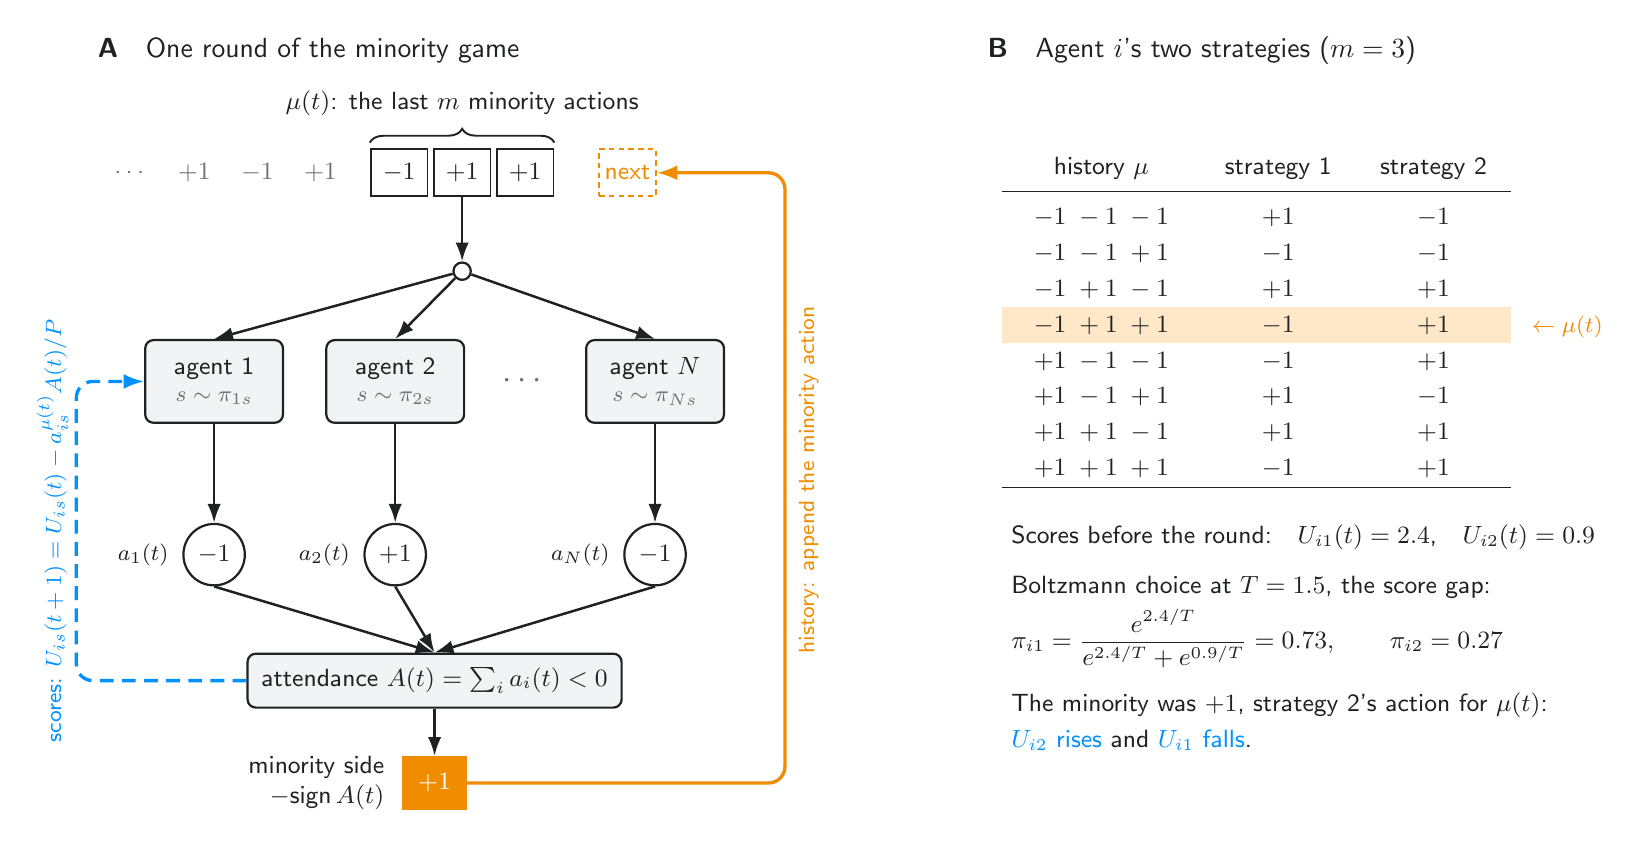
\begin{tikzpicture}
  % ================= Panel A: one round =================
  \node[paneltitle] at (-0.3, 10.85) {\textbf{A}\quad One round of the minority game};

  % the history: older minority actions in gray, the last m = 3 in boxes, the next slot dashed
  \foreach \x/\v in {0.25/\dots, 1.05/$+1$, 1.85/$-1$, 2.65/$+1$} {\node[oldtoken] at (\x, 9.3) {\v};}
  \node[token] (h1) at (3.65, 9.3) {$-1$};
  \node[token] (h2) at (4.45, 9.3) {$+1$};
  \node[token] (h3) at (5.25, 9.3) {$+1$};
  \node[token, draw=saorange, dash pattern=on 2pt off 1.5pt, text=saorange] (next) at (6.55, 9.3) {next};
  \draw[decorate, decoration={brace, amplitude=5pt, raise=2pt}, line width=0.7pt, draw=vnink]
    (h1.north west) -- (h3.north east) node[midway, above=8pt, align=center] {$\mu(t)$: the last $m$ minority actions};

  % the same information goes to every agent
  \node[circle, draw=vnink, fill=white, line width=0.8pt, inner sep=0pt, minimum size=0.22cm] (bc) at (4.45, 8.05) {};
  \draw[flow] (h2.south) -- (bc.north);
  \node[agent] (a1) at (1.3, 6.65) {agent 1\\[-1pt]{\footnotesize\color{gdgray}$s\sim\pi_{1s}$}};
  \node[agent] (a2) at (3.6, 6.65) {agent 2\\[-1pt]{\footnotesize\color{gdgray}$s\sim\pi_{2s}$}};
  \node[text=gdgray, font=\sffamily\large] at (5.25, 6.65) {$\cdots$};
  \node[agent] (aN) at (6.9, 6.65) {agent $N$\\[-1pt]{\footnotesize\color{gdgray}$s\sim\pi_{Ns}$}};
  \foreach \a in {a1, a2, aN} {\draw[flow] (bc) -- (\a.north);}

  % the actions
  \node[action] (x1) at (1.3, 4.45) {$-1$};
  \node[action] (x2) at (3.6, 4.45) {$+1$};
  \node[action] (xN) at (6.9, 4.45) {$-1$};
  \foreach \a/\x in {a1/x1, a2/x2, aN/xN} {\draw[flow] (\a.south) -- ++(0, -0.75) -- (\x.north);}
  \node[anchor=east, font=\sffamily\footnotesize] at (x1.west) {$a_{1}(t)$\,};
  \node[anchor=east, font=\sffamily\footnotesize] at (x2.west) {$a_{2}(t)$\,};
  \node[anchor=east, font=\sffamily\footnotesize] at (xN.west) {$a_{N}(t)$\,};

  % the attendance and the minority side
  \node[sumbox] (sum) at (4.1, 2.85) {attendance $A(t)=\sum_{i}a_{i}(t)<0$};
  \foreach \x in {x1, x2, xN} {\draw[flow] (\x.south) -- (sum.north);}
  \node[minority] (min) at (4.1, 1.55) {$+1$};
  \draw[flow] (sum.south) -- (min.north);
  \node[anchor=east, align=right] at ($(min.west)+(-0.1,0)$) {minority side\\$-\text{sign}\,A(t)$};

  % feedback 1: the minority action becomes the newest entry of the history
  \draw[feedback] (min.east) -- (8.55, 1.55) -- (8.55, 9.3) -- (next.east);
  \node[rotate=90, text=saorange, font=\sffamily\footnotesize] at (8.85, 5.4) {history: append the minority action};
  % feedback 2: the attendance updates every strategy's score
  \draw[scorefeed] (sum.west) -- (-0.45, 2.85) -- (-0.45, 6.65) -- (a1.west);
  \node[rotate=90, text=gdblue, font=\sffamily\footnotesize] at (-0.75, 4.75) {scores: $U_{is}(t+1)=U_{is}(t)-a_{is}^{\mu(t)}A(t)/P$};

  % ================= Panel B: one agent's strategies =================
  \begin{scope}[xshift=11.3cm]
    \node[paneltitle] at (-0.3, 10.85) {\textbf{B}\quad Agent $i$'s two strategies ($m=3$)};
    \node[anchor=north west, inner sep=0pt] at (0.0, 9.6) {%
      \renewcommand{\arraystretch}{1.18}%
      \begin{tabular}{>{\centering\arraybackslash}p{2.1cm}>{\centering\arraybackslash}p{1.55cm}>{\centering\arraybackslash}p{1.55cm}l}
        history $\mu$ & strategy 1 & strategy 2 & \\[2pt] \cline{1-3}
        \rule{0pt}{12pt}$-1\;-1\;-1$ & $+1$ & $-1$ & \\
        $-1\;-1\;+1$ & $-1$ & $-1$ & \\
        $-1\;+1\;-1$ & $+1$ & $+1$ & \\
        \cellcolor{orangefill}$-1\;+1\;+1$ & \cellcolor{orangefill}$-1$ & \cellcolor{orangefill}$+1$ & \textcolor{saorange}{\footnotesize\bfseries\,$\leftarrow\mu(t)$} \\
        $+1\;-1\;-1$ & $-1$ & $+1$ & \\
        $+1\;-1\;+1$ & $+1$ & $-1$ & \\
        $+1\;+1\;-1$ & $+1$ & $+1$ & \\
        $+1\;+1\;+1$ & $-1$ & $+1$ & \\ \cline{1-3}
      \end{tabular}};

    % scores, probabilities, and the update after this round
    \node[anchor=north west, align=left] at (0.0, 4.95) {%
      Scores before the round:\quad $U_{i1}(t)=2.4$,\quad $U_{i2}(t)=0.9$\\[7pt]
      Boltzmann choice at $T=1.5$, the score gap:\\[3pt]
      $\pi_{i1}=\dfrac{e^{2.4/T}}{e^{2.4/T}+e^{0.9/T}}=0.73,\qquad \pi_{i2}=0.27$\\[8pt]
      The minority was $+1$, strategy 2's action for $\mu(t)$:\\[2pt]
      \textcolor{gdblue}{$U_{i2}$ rises} and \textcolor{gdblue}{$U_{i1}$ falls}.};
  \end{scope}
\end{tikzpicture}
\end{document}
